\chapter{Supplementary Material}
\section*{Infrastructure}
Model Architecture: UNET 2D and 3D

Trained on A100 GPU 80 GB using Maxwell Cluster at DESY. 

\section{Results}

\begin{figure}
    \centering
    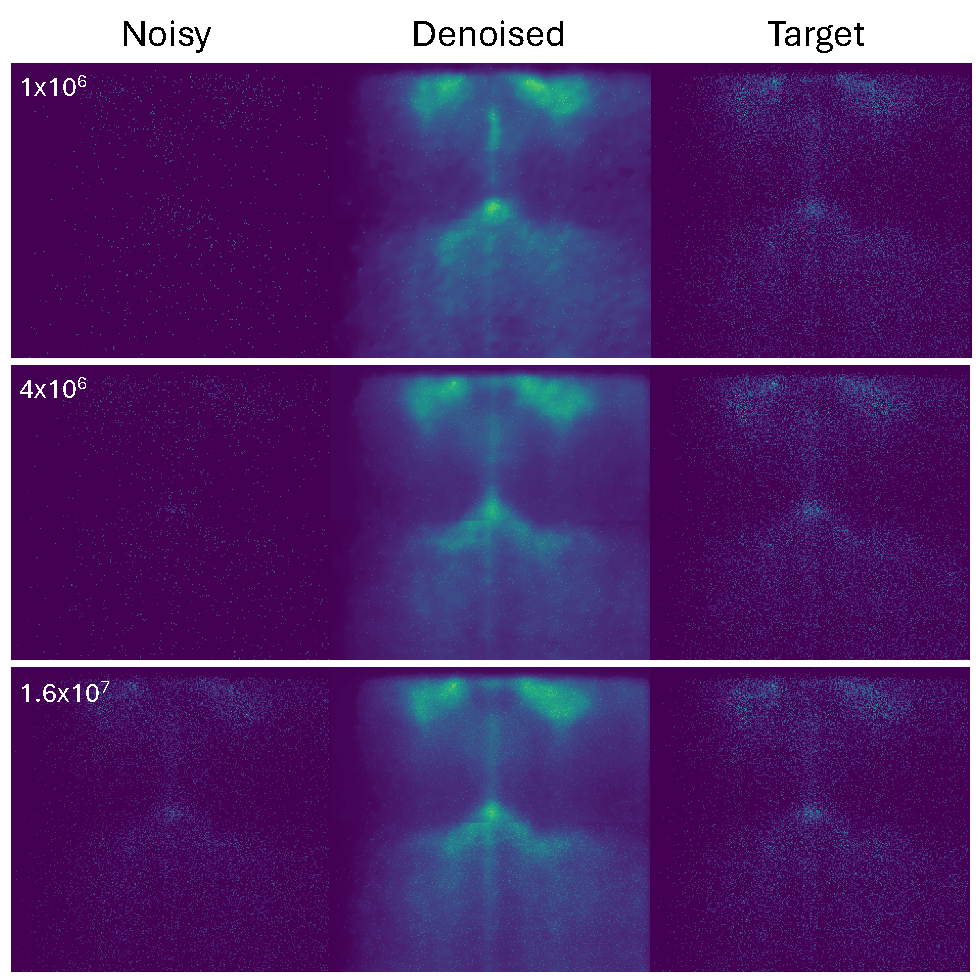
\includegraphics[width=1\linewidth]{images/nn_denoised_ex_single_slice.pdf}
    \caption{Noisy, denoised, and target \gls{E}-\gls{kx} cuts with window size $w=1$ shown for \gls{GdW} dataset. Each row corresponds \numlist{1e6;4e6;1.6e7} counts, respectively.}
    \label{fig:nn-denoised-ex-single-slice}
\end{figure}

\begin{figure}
    \centering
    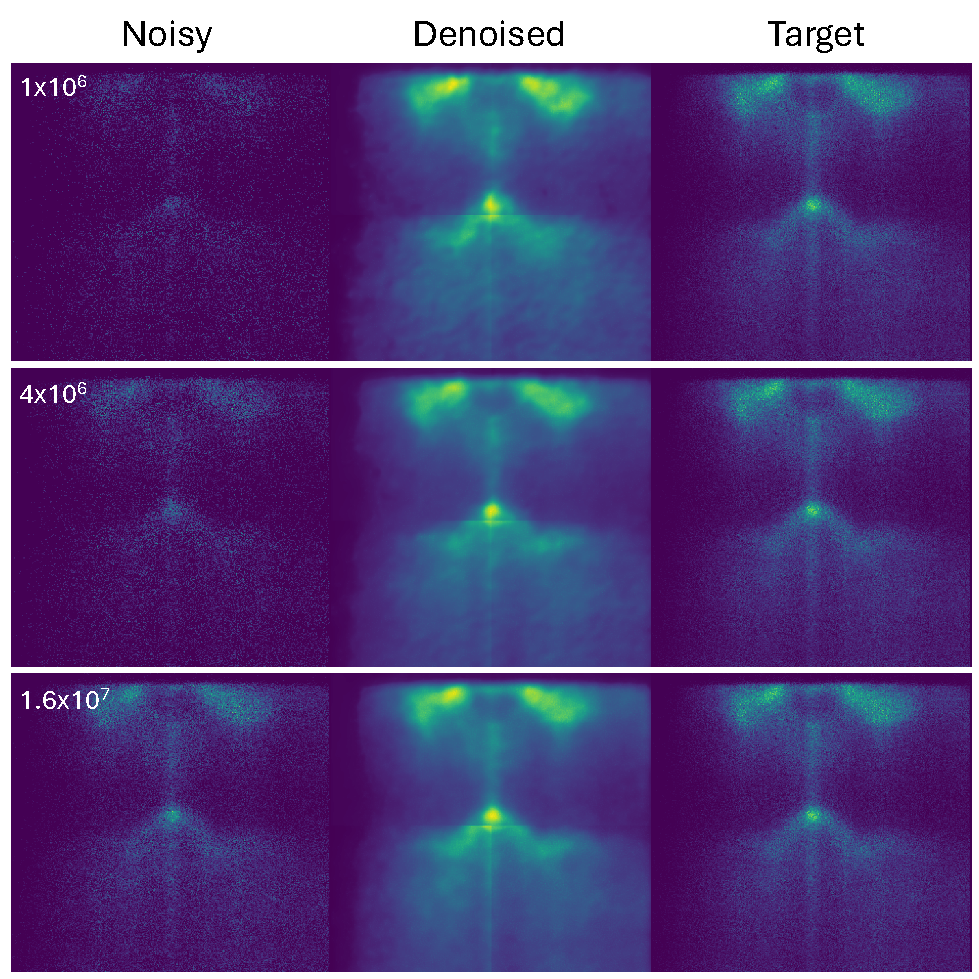
\includegraphics[width=1\linewidth]{images/nn_denoised_ex_20_slice.pdf}
    \caption{Noisy, denoised, and target \gls{E}-\gls{kx} cuts with window size $w=20$ shown for \gls{GdW} dataset. Each row corresponds \numlist{1e6;4e6;1.6e7} counts, respectively.}
    \label{fig:nn-denoised-ex-20-slice}
\end{figure}

\begin{figure}
    \centering
    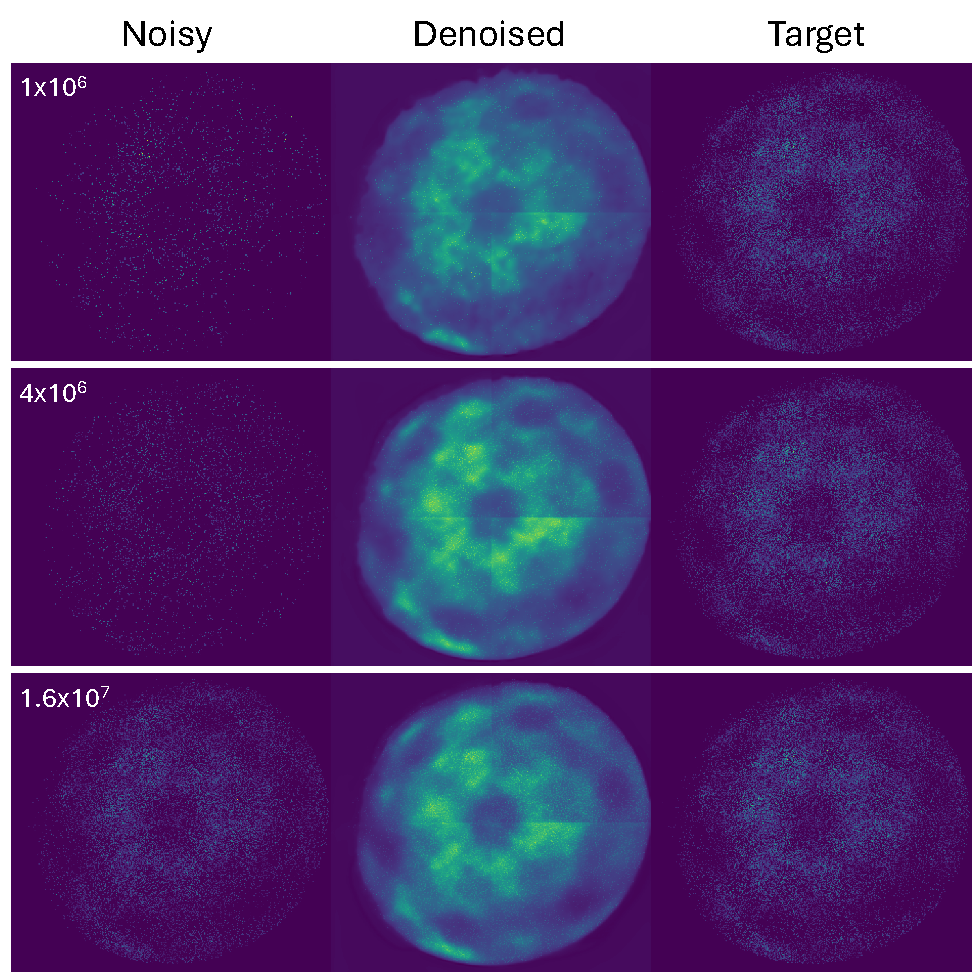
\includegraphics[width=1\linewidth]{images/nn_denoised_xy_single_slice.pdf}
    \caption{Noisy, denoised, and target \gls{ky}-\gls{kx} cuts with window size $w=1$ shown for \gls{GdW} dataset. Each row corresponds \numlist{1e6;4e6;1.6e7} counts, respectively.}
    \label{fig:nn-denoised-xy-single-slice}
\end{figure}

\begin{figure}
    \centering
    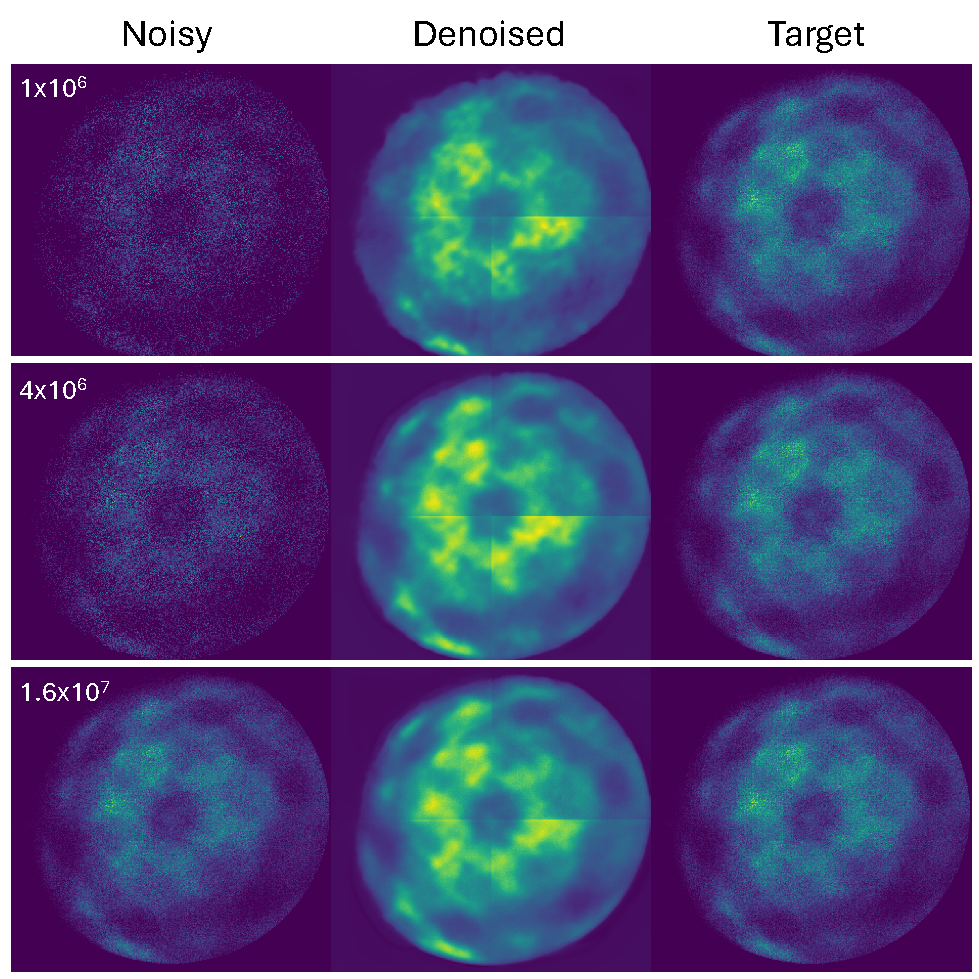
\includegraphics[width=1\linewidth]{images/nn_denoised_xy_20_slice.pdf}
    \caption{Noisy, denoised, and target \gls{ky}-\gls{kx} cuts with window size $w=20$ shown for \gls{GdW} dataset. Each row corresponds \numlist{1e6;4e6;1.6e7} counts, respectively.}
    \label{fig:nn-denoised-xy-20-slice}
\end{figure}

\section{Supplementary Figures for Photoelectron Counting Statistics}
The following section outlines the counting statistics observed for \gls{PES} at two different light sources: a pulsed laser (\gls{WSe2} dataset), and a \gls{SASE} \gls{FEL} light source (\gls{GrIr} dataset). 

\cref{fig:wse2-stats-2} shows the distribution of photoelectron counts for different time intervals ($\Delta t$) within a volumetric subset of the full \gls{WSe2} dataset. The count distributions for smaller time intervals ($\Delta t = \qtylist{2;10;20}{ms}$) follow Poisson statistics, as expected from an uncorrelated photoemission process where spatial and temporal fluctuations are minimal. However, for longer time intervals ($\Delta t = \qty{50}{ms}$), the distribution starts to deviate from the Poisson distribution. This deviation suggests that spatial correlations, due to the material properties of the sample, become significant enough to impact the distribution. While the impact of pulse light source should be minimal since the time intervals we look at are much longer than the pulse durations, the spatial correlations could be due to the material properties of the sample.


The \gls{GrIr} dataset reveals more complex photoelectron count statistics over a broader range of time intervals. Figures \ref{fig:grir-stats-1}, \ref{fig:grir-stats-2}, and \ref{fig:grir-stats-3} show photoelectron count distributions for varying time windows ($\Delta t = \qtylist{10;50;100;500;1000;5000}{ms}$) in the acquisition time $T\approx\qty{30}{hour}$


\begin{figure}
    \centering
    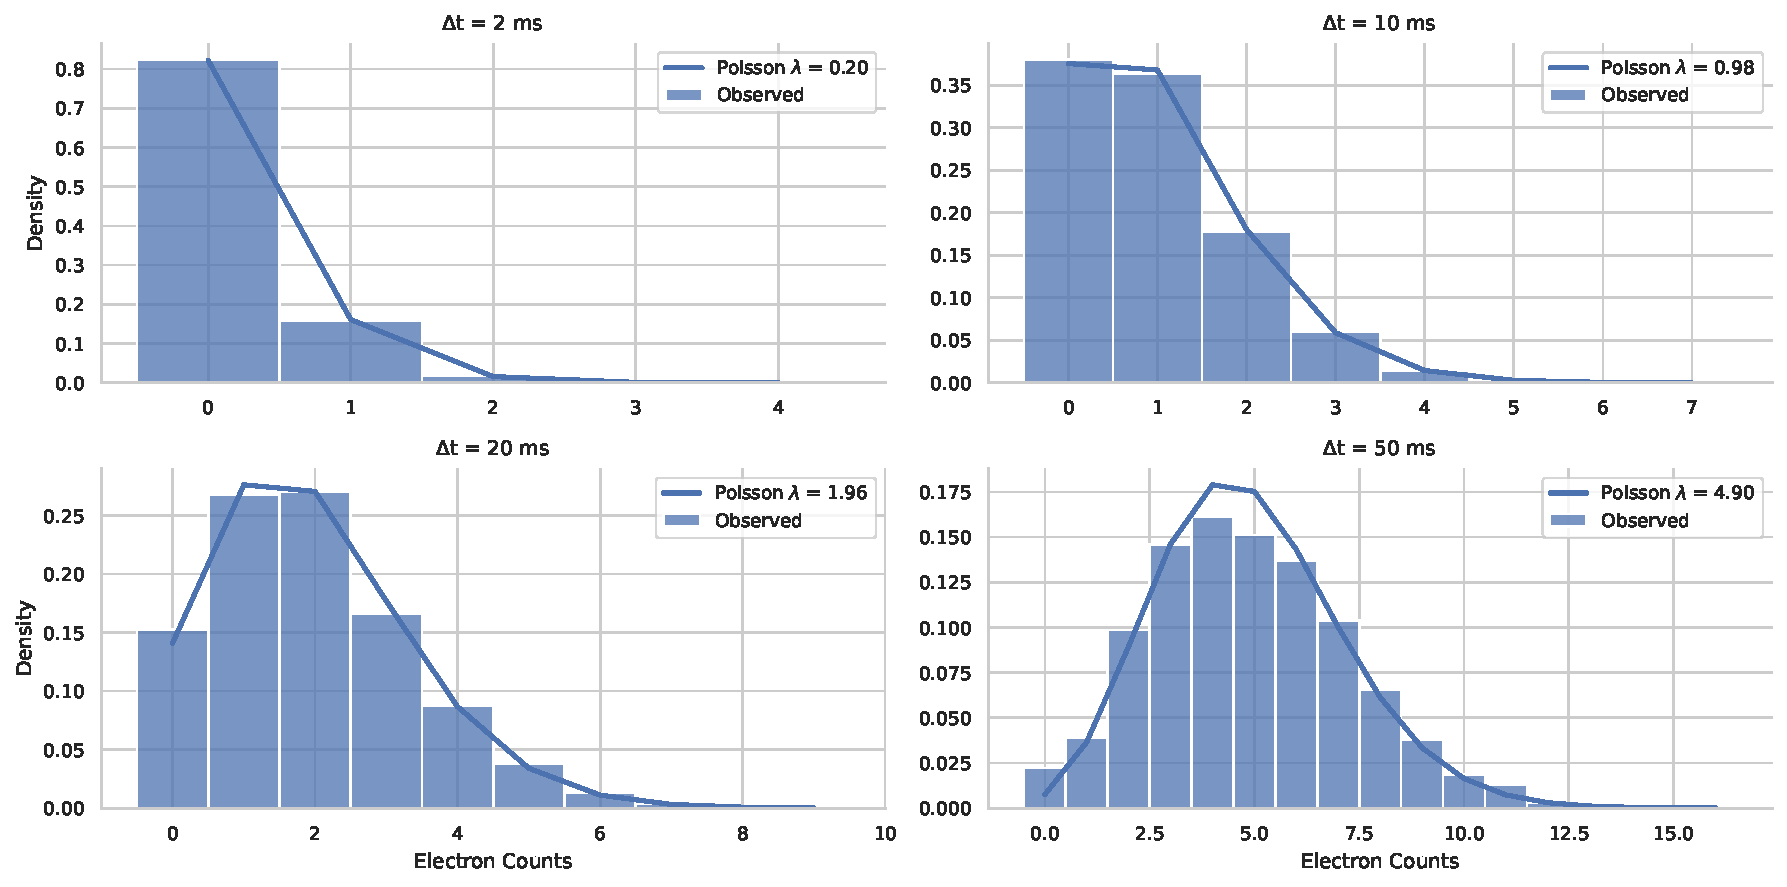
\includegraphics[width=1\linewidth]{images/hist_counts_facetgrid_2_wse2.pdf}
    \caption{Distribution of photoelectron counts at time intervals $\Delta t =$ \qtylist{2;10;20;50}{ms} for a different volumetric subset of the full \gls{WSe2} dataset. Poisson statistics are observed at smaller time intervals, but as the time window increases ($\Delta t =$ \qty{50}{ms}), the data starts to deviate from the Poisson distribution, as spatial correlations become apparent.}
    \label{fig:wse2-stats-2}
\end{figure}





\begin{figure}
    \centering
    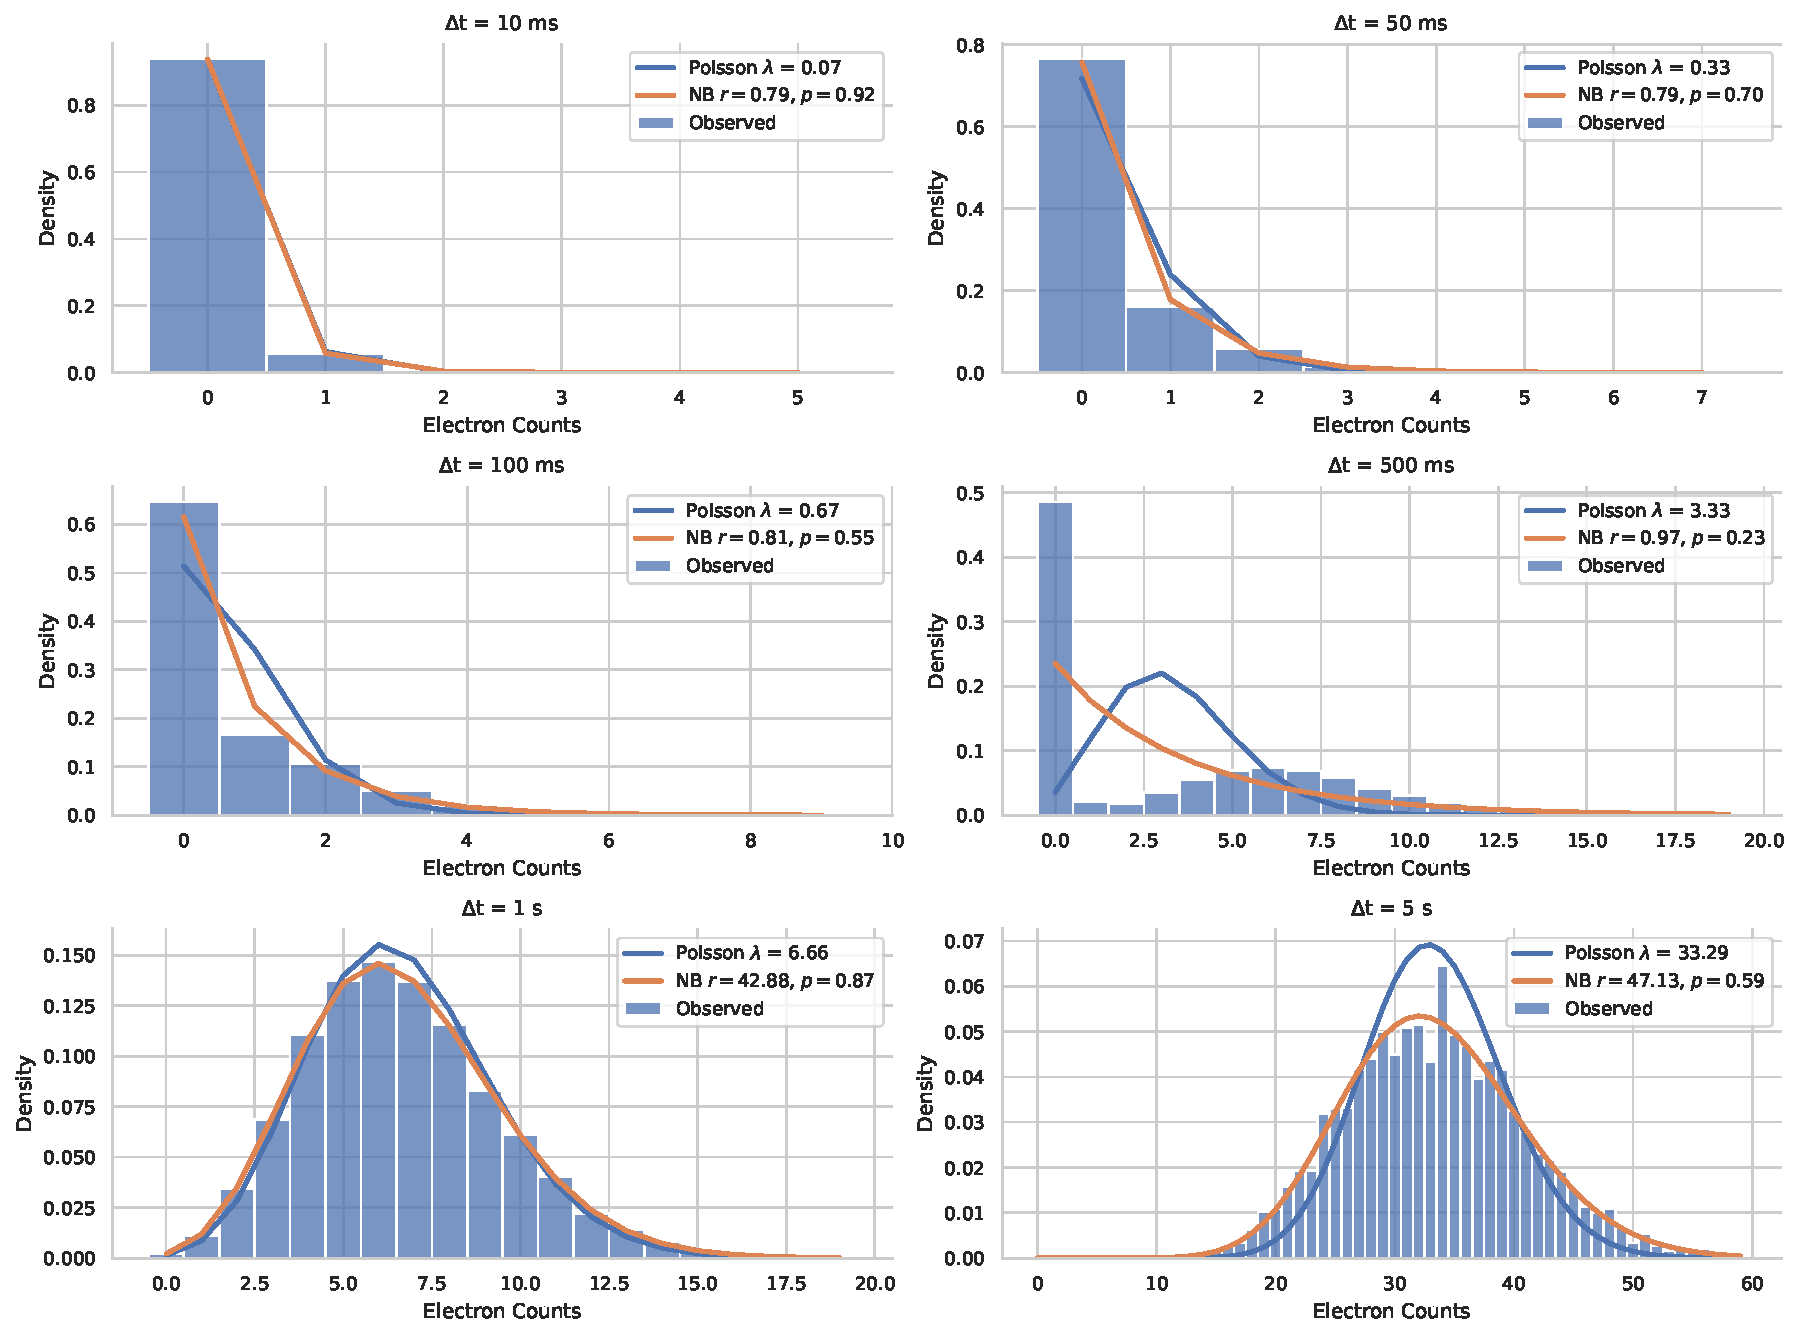
\includegraphics[width=1\linewidth]{images/hist_counts_facetgrid_3_grir.pdf}
    \caption{Distribution of photoelectron counts at time intervals $\Delta t =$ \qtylist{10;50;100;500;1000;5000}{ms} for a selected volumetric subset of the full \gls{GrIr} dataset. Poisson statistics provide a good fit at $\Delta t \leq \qty{100}{ms}$. However, for intervals $\Delta t =$ \qtylist{0.5;1;5}{s} the distribution exhibits over dispersion with a right-skewed tail, characteristic of the \gls{NB} distribution. The total counts in this selected region are $\gls{ncounts}=\num{1e6}$ with total observation time $T\approx\qty{4}{h}$  (See red region in \cref{fig:gmd-intensity}). The smaller $\Delta t$ values may represent the limiting case of the \gls{NB} distribution approaching Poisson statistics.}
    \label{fig:grir-stats-3}
\end{figure}